\chapter{Validation Test Cases}
\label{cha:tests}


\section{Introduction}

In order to validate the developed coupling adapter, several test cases were simulated, which ought to
qualitatively and quantitatively confirm the physically correct implementation. Moreover, the capabilities
of the adapter for larger-scale two- as well as three-dimensional simulations are shown in the following.
All simulations in this chapter were carried out on the MAC Cluster "CoolMAC" using the "Sandybridge"
and "Bulldozer" partitions1. The coupled structural solver for all simulations was the module SOLIDZ
(CSM simulations), which is part of the multiphysics simulation software suite Alya that is developed
at the Barcelona Supercomputing Center ([44]). Meshes for the testcases were generated with the free
software Gmsh ([19]).
Each section in this chapter starts with a short definition of the respective testcase, including its geometry,
discretization, expectation of the physical behavior and a motivation for running the simulation.
Subsequently, I state the physical and numerical settings used for the run. In the end, the obtained
results are shown and discussed briefly.
Beginning with Section 6.1, a very simple two-dimensional testcase is described, which is altered to yield a
three-dimensional scenario in Section 6.2. A quantitative comparison of simulation results is possible via
running the well-known FSI3 benchmark testcase ([39]) in Section 6.3. The chapter is closed by Section
6.4, simulating a slender cylinder. This example has a practical background and represents a real-world
application.
As for all simulations material and physical parameters as well as solver configurations need to be defined,
I forestall them here in order to avoid repeating myself in each section of this chapter. Also, this allows
to compare simulations settings with each other more easily. Material and physical parameters are stated
in Table 6.1. Fluids are modeled as ideal gases, solids as linearly elastic and isotropic.
Several solver configuration options remain the same for all simulations: Forces and the displacements
relative to the last time step are chosen as coupling quantities. In case an implicit coupling algorithm is
used, these are monitored by preCICE for convergence of the fixed-point system. In addition, an implicit
coupling algorithm extrapolates the coupling quantities with a second-order scheme at the beginning of
each time step. If IQN-ILS or V-IQN (recall Section 4.1.1) are chosen for coupling, preCICE takes into
account up to 30 iterations of up to 10 previous time steps in order to solve the interface least-squares
problem.
Concerning SU2, time discretization is handled by the implicit Euler method and spatial discretization is
dealt with by a second-order scheme in combination with a Roe approximate Riemann solver ([34]). The
linear system, which finally yields the solution vector of the flow field, is solved by the FGMRES procedure
([35]). All other solver configurations are given in Table 6.2 or directly stated in the respective sections.
Note that some FSI simulations are initialized from a fluid-only start solution, which is calculated for a
time period specified with tstart. Also, some simulations make use of the dual time stepping technique of
%SU2. The corresponding dual time convergence limit dual relates to reducing the density residual of the
fluid domain.
Fluid and solid calculations are started on different nodes of the cluster for all simulations.



\section{Dummy fluid solver}

The first task implemented to validate the adapter consisted in developing a simple \textit{dummy fluid solver}: i.e. a software component connected to the coupling library preCICE with the simple task to apply forces to user-defined nodes on the structure and read back the displacements.

This approach allowed to validate first to validate the MBDyn model with the \texttt{external structural mapping} component (see Section \ref{sec:mbd-forces}) and the correct data exchange between preCICE and the adapter. 

The \textit{dummy solver} has been written in Python and it is part of the software package in this work.

A MBDyn model composed of 5 \texttt{beam3} elements (see Section \ref{sec:mbd-beam}) has been written to perform this test, as depicted in Figure \ref{fig:cnt-beams}. The beam section is constant and rectangular and the physical properties are constant throughout the beam length. 

\begin{figure}[htbp!]
	    \centering
        \begin{tikzpicture}
            \point{a}{0}{0};
            \point{b}{1.5}{0};
            \point{c}{3}{0};
            \point{d}{4.5}{0};
            \point{e}{6}{0};
            \point{f}{7.5}{0};
            
            \beam{4}{a}{b};
            \beam{4}{b}{c};
            \beam{4}{c}{d};
            \beam{4}{d}{e};
            \beam{4}{e}{f};
            
            \notation{2}{b}{};
            \notation{2}{c}{};
            \notation{2}{d}{};
            \notation{2}{e}{};
            \notation{2}{f}{};
            
            \notation{4}{a}{b}[ $1$ ];
            \notation{4}{b}{c}[ $2$ ];
            \notation{4}{c}{d}[ $3$ ];
            \notation{4}{d}{e}[ $4$ ];
            \notation{4}{e}{f}[ $5$ ];
            
            \support{3}{a}[-90]
            % \load{1}{b}[90][1][.1];
            \dscaling{3}{0.5};
            \daxis{1}{-1.5 ,0 ,0}[right][above][left];
        \end{tikzpicture}
    	\caption{cantilever made of 5 beam elements}
		\label{fig:cnt-beams}
\end{figure}

The inertia of the structure is provided by 2 \texttt{body} elements (see Section \ref{sec:mbd-body} attached to the second and third nodes of each beam (see Figure \ref{fig:mbdyn-beam-model}). The center of gravity of each body is offset by $-l/4$ in x-direction (where $l$ is the length of the single beam element). Each body has the following inertial properties (see Figure \ref{fig:cnt-mass}: 

\begin{equation}
    m = \rho A \frac{l}{4} \quad I = \frac{m}{12} \begin{bmatrix} h^2+w^2 & 0 & 0 \\ 0 & \frac{l^2}{16} + w^2 & 0 \\ 0 & 0 & \frac{l^2}{16} + h^2 \end{bmatrix}
    \label{eq:body-inertia}
\end{equation}


\begin{figure}[htbp!]
	    \centering
\begin{tikzpicture}[every edge quotes/.append style={auto, text=blue}]
  \pgfmathsetmacro{\cubex}{4}
  \pgfmathsetmacro{\cubey}{2}
  \pgfmathsetmacro{\cubez}{3}
  \draw [draw=blue, every edge/.append style={draw=blue, densely dashed, opacity=.5}, fill=yellow!10]
    (0,0,0) coordinate (o) -- ++(-\cubex,0,0) coordinate (a) -- ++(0,-\cubey,0) coordinate (b) edge coordinate [pos=1] (g) ++(0,0,-\cubez)  -- ++(\cubex,0,0) coordinate (c) -- cycle
    (o) -- ++(0,0,-\cubez) coordinate (d) -- ++(0,-\cubey,0) coordinate (e) edge (g) -- (c) -- cycle
    (o) -- (a) -- ++(0,0,-\cubez) coordinate (f) edge (g) -- (d) -- cycle;
  \path [every edge/.append style={draw=black, |-|}]
    (b) +(0,-5pt) coordinate (b1) edge ["$l/2$"] (b1 -| c)
    (b) +(-5pt,0) coordinate (b2) edge ["h"] (b2 |- a)
    (c) +(3.5pt,-3.5pt) coordinate (c2) edge ["w"] ([xshift=3.5pt,yshift=-3.5pt]e)
    ;
    \daxis{1} {-8,-1,-1.5} [right][above][left];
    \dpoint{q}{-2.5}{-1}{-1.5};
    \dpoint{r}{0}{-1}{-1.5};
    \dpoint{s}{-\cubex}{-1}{-1.5};
    \dpoint{t}{\cubex}{-1}{-1.5};
    \beam{4}{q}{r};
    \dhinge{1}{q};
    \dhinge{1}{r};
    \dhinge{1}{s};
    \dhinge{1}{t};
    \dnotation{1}{q}{CoG};
    \dnotation{1}{r}{$n_2$};
    \dnotation{1}{s}{$n_1$};
    \dnotation{1}{t}{$n_3$};
    \ddimensioning{xy}{q}{r}{1.5}[ $l/4$ ];
    \ddimensioning{xy}{s}{t}{-2.5}[ $l$ ];
    
\end{tikzpicture}
    	\caption{\texttt{body} element attached to node 2 of the \texttt{beam} element}
		\label{fig:cnt-mass}
\end{figure}


The interface mesh is represented in Figure \ref{fig:mbdyn-mesh}.


\begin{figure}[htbp!]
	\centering
	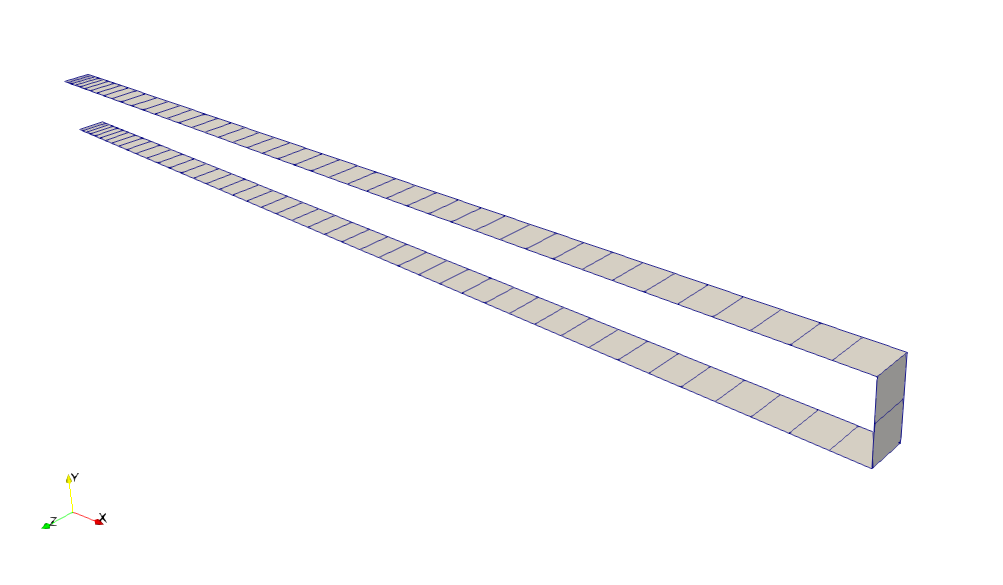
\includegraphics[width=0.7\textwidth]{images/example-mesh}
	\caption{interface points mesh}
	\label{fig:mbdyn-mesh}
\end{figure}

The model has been loaded by a concentrated load on the tip (Figure \ref{fig:cnt-tip} and with an equivalent distributed load on the upper surface (Figure \ref{fig:cnt-distrib}).

\begin{figure}[htbp!]
	%\centering
	    \begin{subfigure}{.8\textwidth}
	    \centering
        \begin{tikzpicture}
            \point{a}{0}{0};
            \point{b}{6}{0};
            \beam{4}{a}{b};
            \support{3}{a}[-90]
            \load{1}{b}[90][1][.1];
        \end{tikzpicture}
    	\caption{cantilever with tip load}
		\label{fig:cnt-tip}
	    \end{subfigure}
	    %\newline
	    \par\bigskip
	    \begin{subfigure}{.8\textwidth}
		\centering
		\begin{tikzpicture}
            \point{a}{0}{0};
            \point{b}{6}{0};
            \beam{4}{a}{b};
            \support{3}{a}[-90]
            \lineload{1}{a}{b}[1][1];%[force interval];
        \end{tikzpicture}
    	\caption{cantilever with distributed load}
		\label{fig:cnt-distrib}
	    \end{subfigure}
	\caption{model and data exchange test-cases}
\end{figure}

The results have been compared the expected values in terms of tip displacement at steady state and in terms of frequency of the tip movement when the system has been loaded with a step load.

When both the MBDyn model and the data exchanged through the preCICE interface have been validated, the model has been coupled to a CFD solver.

\section{Vertical flap: incompressible regime}

\section{Vertical flap: compressible regime}


\section{Square cylinder Benchmark}


\cite{ramm1998fluid} art originale.
\cite{walhorn2002space}
\cite{matthies2003partitioned}
\cite{dettmer2006computational}
\cite{olivier2009fluid}
\cite{wood2010partitioned}
\cite{kassiotis2011nonlinear}
\cite{habchi2013partitioned}
\cite{froehle2014high}


\section{Turek-Hron FSI2 Benchmark}



\section{Turek-Hron FSI1 and FSI3 Benchmark}


\section{Sensitivity analysis of FSI3 Benchmark}




